\documentclass[a4paper,11pt,twoside]{article}
\usepackage[T1]{fontenc}
\usepackage[utf8]{inputenc}
\usepackage{ngerman, eucal, mathrsfs, amsfonts, bbm, amsmath, amssymb, stmaryrd,graphicx, array, geometry, listings, color}
\geometry{left=25mm, right=15mm, bottom=25mm}
\setlength{\parindent}{0em} 
\setlength{\headheight}{0em} 
\title{Machine Learning\\ Blatt 1}
\author{Markus Vieth, David Klopp, Christian Stricker}
\date{\today}
\newcommand{\limesS}{\text{lim sup}}
\newcommand{\lsi}{\limesS_{n\rightarrow \infty}} %lim sup n nach inf
\newcommand{\limesinf}{\text{lim}_{n\rightarrow \infty}}


\begin{document}

\maketitle
\cleardoublepage
\pagestyle{myheadings}
\markboth{Markus Vieth,  David Klopp, Christian Stricker}{Markus Vieth, David Klopp, Christian Stricker}

\section*{Nr.1}

\subsection*{a)}
\begin{figure}[h]
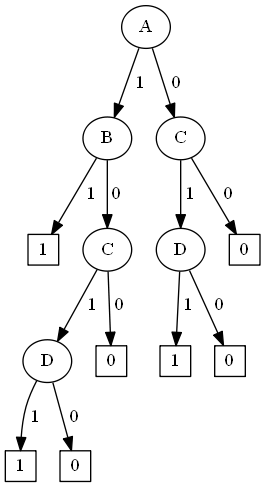
\includegraphics[width=0.3\textwidth]{Aufgabe1/graphA.png}
\end{figure}

\subsection*{b)}
\begin{figure}[h]
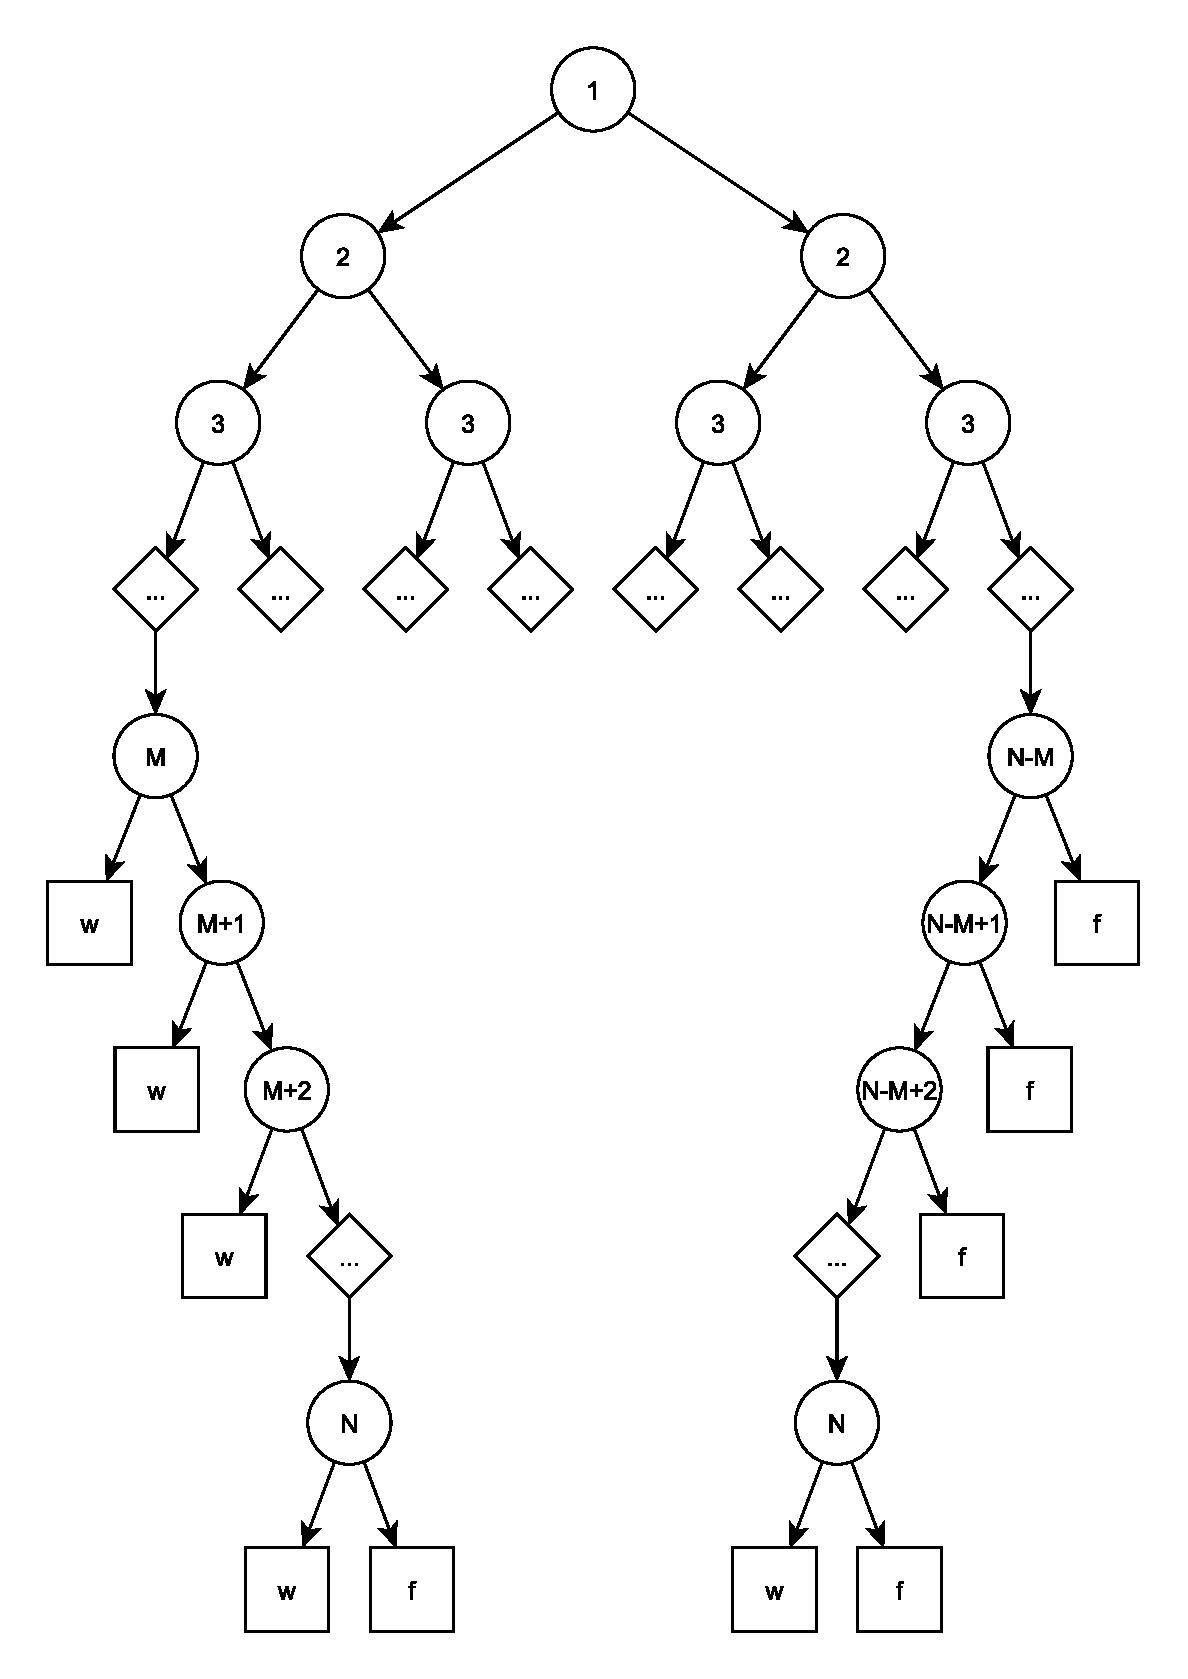
\includegraphics[width=0.6\textwidth]{Aufgabe1/graphB.eps}
\end{figure}

\newpage

\section*{Nr.3}
\subsection*{a)}
$S = \{A,B,C,D\}$ 
\[ H(S) = -p(A)log2(p(A))-p(B)log2(p(B))-p(C)log2(p(C))-p(D)log2(p(D)) \]
\[ = -0,5*log2(0,5)-0,3*log2(0,3)-0,1*log2(0,1)-0,1*log2(0,1) \]
\[ = 1.685475297227334319499038031560350135304471374204545987890...\]

\subsection*{b)}
$max = log2(|S|)~~,\forall x \in S ~~~\text{gilt:}~~~ p(x) = 1/|S|$\\
$min = 0 \Leftrightarrow \exists x \in S ~~~\text{mit}~~~ p(x) = 1  \Rightarrow \forall y \in S \setminus \{x\} : p(y) = 0$

\subsection*{c)}
Entropie ist eine Skala für die Verteilung der Werte des Klassenattributes auf die Werte des betrachteten Attributes. Somit bedeutet eine niedrige Entropie, dass sich die Werte des Klassenattributes auf einige wenige Werte des betrachteten Attributes verteilen, wo hingegen eine hohe Entropie bedeutet, dass sich die Werte des Klassenattributes gelichmäßig auf die Werte des betrachteten Attributes verteilen.

\subsection*{d)}
Bei einem Entscheidungsbaum ist die Reihenfolge der Betrachtung der Attribute für dessen Komplexität von Bedeutung. Die Qualität eines Attributes kann mithilfe des InformationGains bewertet werden. Dazu betrachten wir die erwartete Verminderung der aktuellen Entropie bei Wahl des betrachteten Attributes. Durch eine niedrige erwartete Entropie wird der Baum kürzer.


\section*{Nr.5}


\end{document}